\documentclass[11pt]{article}
\usepackage[margin=1in]{geometry}
\usepackage{enumerate,graphicx}
\title{Cookbook}
\author{Collin Cappelle}

\begin{document}
\maketitle
\pagebreak
\tableofcontents
\pagebreak

\section{Potatoes}
\subsection{Potato Pancakes}
Date Created: November 13, 2016

\subsubsection*{Ingredients}
\begin{itemize}
	\item 2 medium sized russet potatoes
	\item 1/2 of an onion
	\item 1 large egg
	\item 1.5 Tbls of flour
	\item Vegetable oil
\end{itemize}
\subsubsection*{Method}
\begin{enumerate}
	\item Shred potatoes and onion into a bowl of cold water. Let sit for 20-30 minutes.
	\item Mix egg, flour, salt, cayenne pepper, and black pepper in a seperate bowl.
	\item Drain potatoes and squeeze out excess water until dry.
	\item Mix potatoes into egg mixture.
	\item Heat 1/2" of oil in a pan on medium-high
	\item Form potato pancakes and place in oil
	\item Cook for 5-8 minutes on each side until browned
	\item Let drain on rack to get rid of excess oil
\end{enumerate}
\subsubsection*{Notes and Result}
Pancakes were well cooked. Nice crisp on the outside with a strong onion flavor on the inside. A little bit greasy so either wait for hotter oil or make bigger patties.\\
\begin{center}
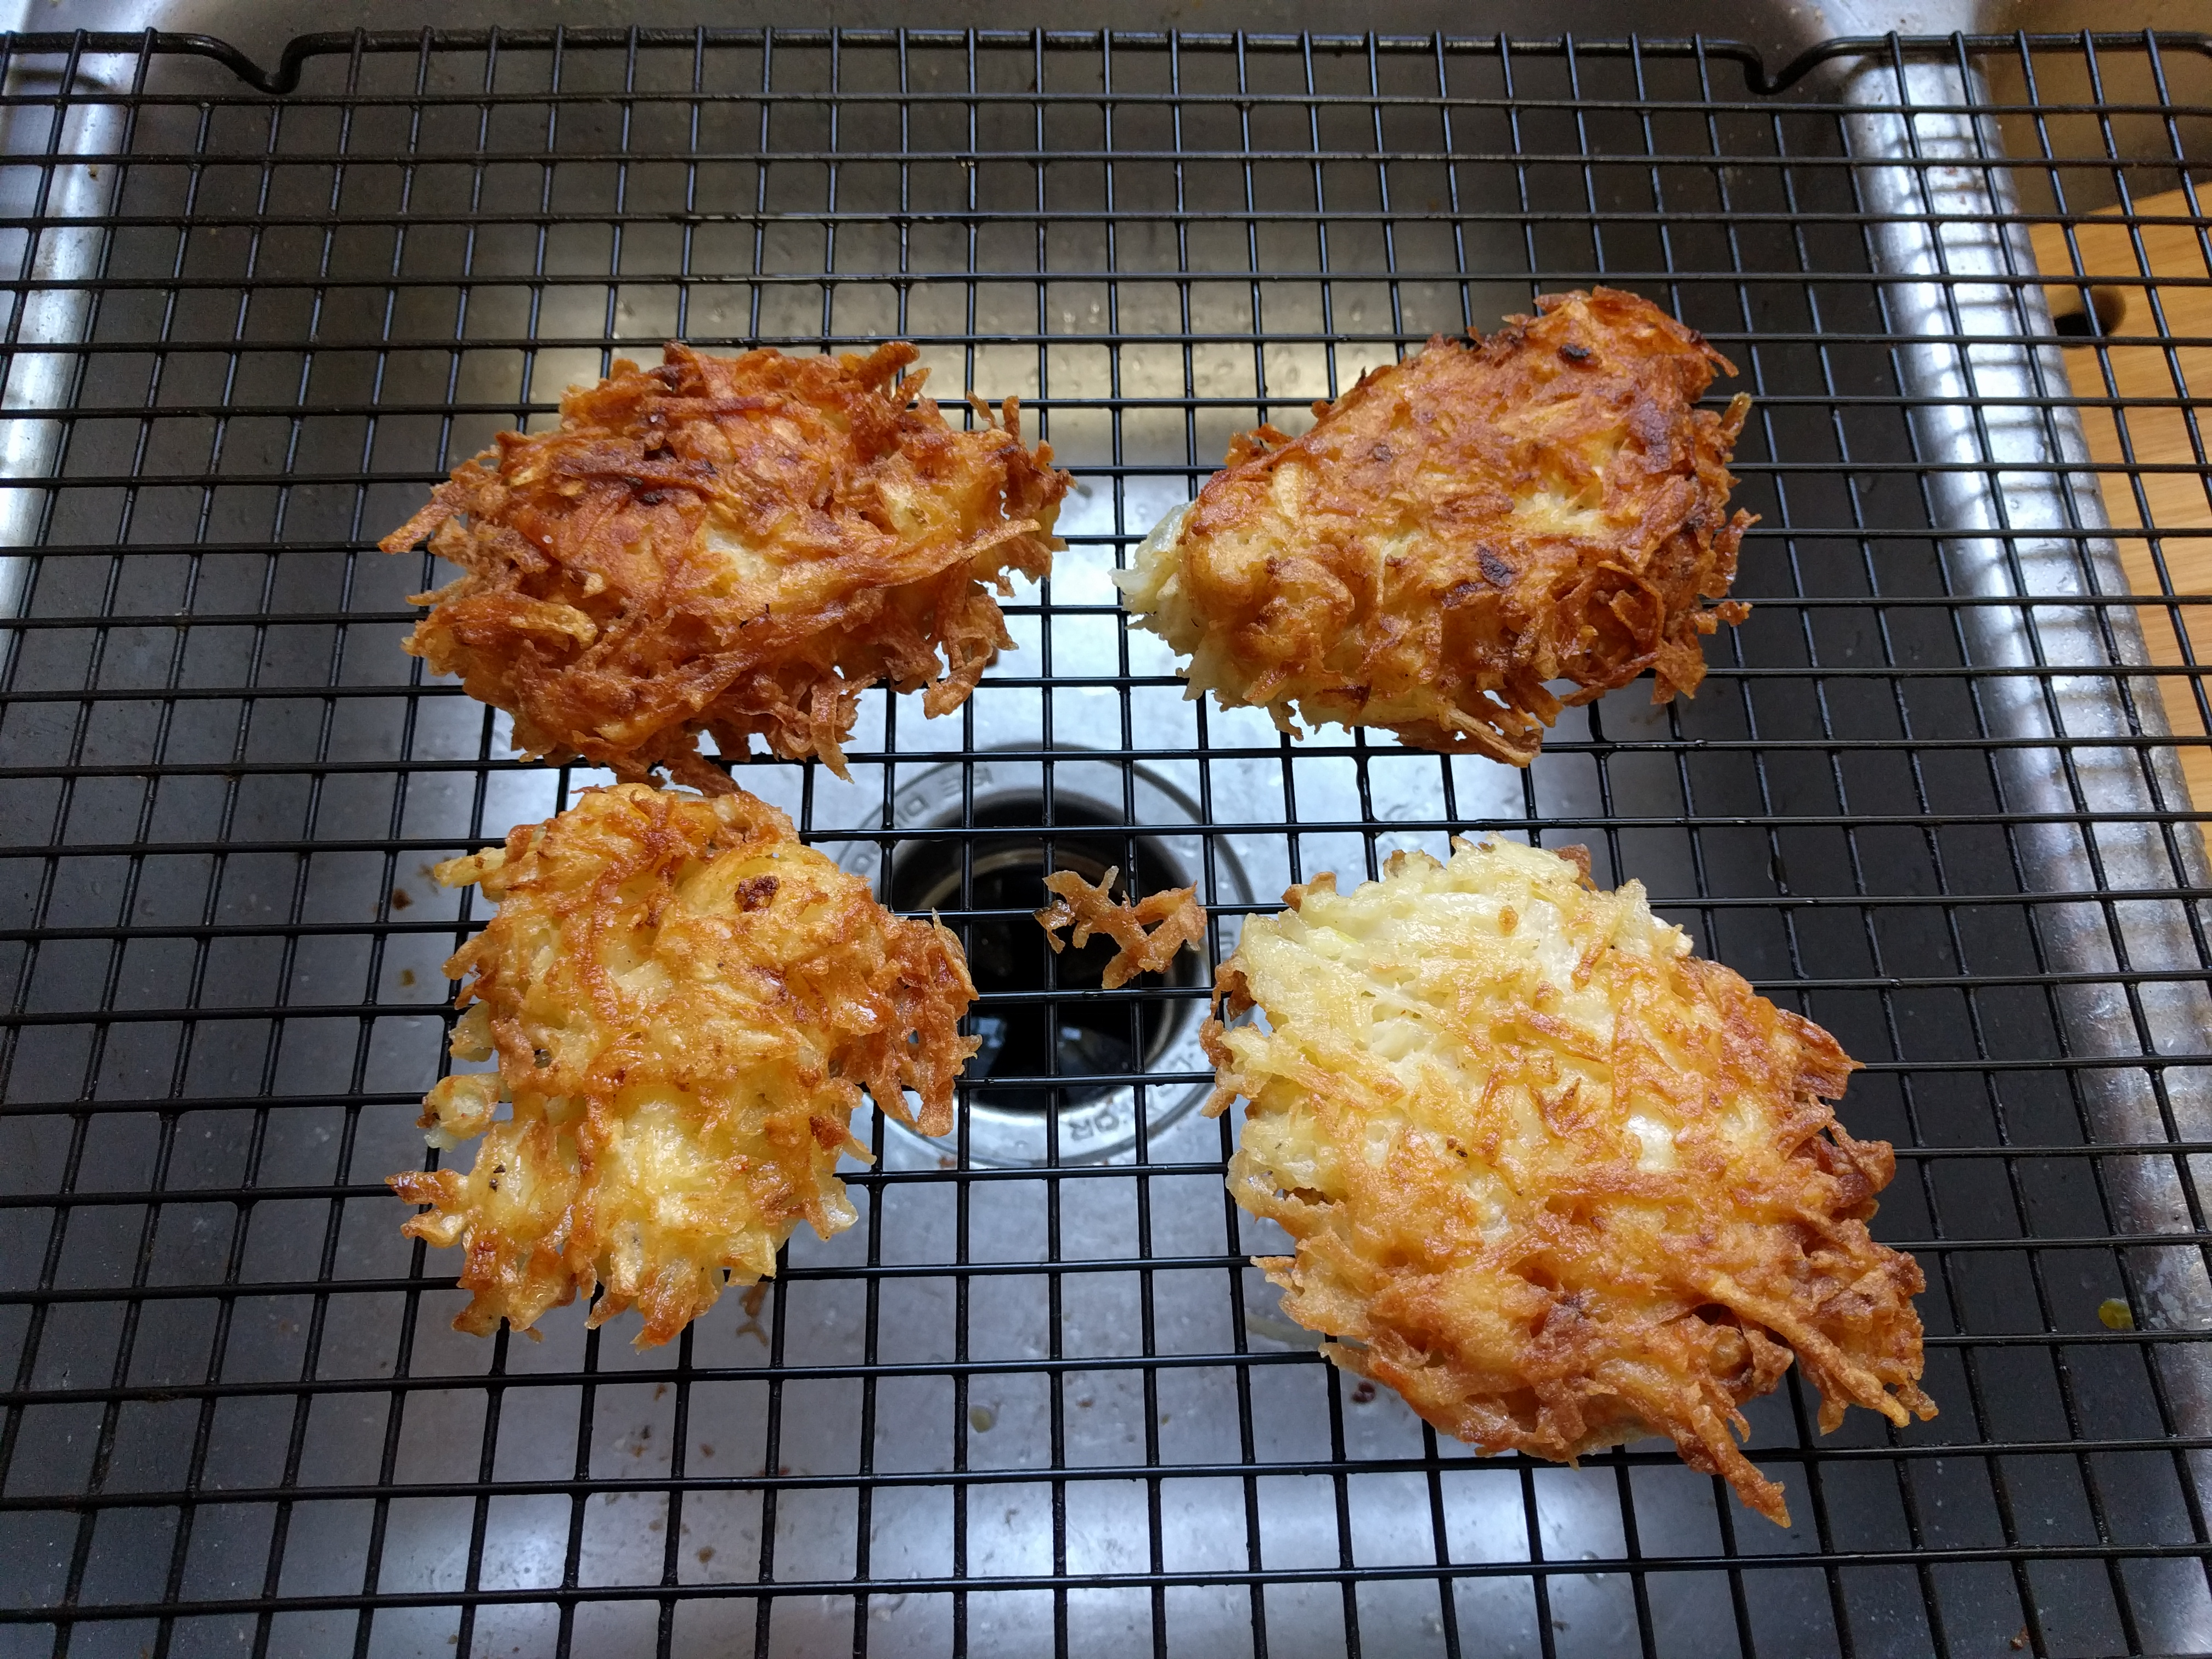
\includegraphics[width=.5\linewidth]{2016-11-13-Potato_Pancakes.jpg}
\end{center}
\end{document}